%%%%%%%% ICML 2018 EXAMPLE LATEX SUBMISSION FILE %%%%%%%%%%%%%%%%%

\documentclass{article}

% Recommended, but optional, packages for figures and better typesetting:
\usepackage{microtype}
\usepackage{graphicx}
\usepackage{subfigure}
\usepackage{booktabs} % for professional tables

% hyperref makes hyperlinks in the resulting PDF.
% If your build breaks (sometimes temporarily if a hyperlink spans a page)
% please comment out the following usepackage line and replace
% \usepackage{icml2018} with \usepackage[nohyperref]{icml2018} above.
\usepackage{hyperref}

% Attempt to make hyperref and algorithmic work together better:
\newcommand{\theHalgorithm}{\arabic{algorithm}}

% Use the following line for the initial blind version submitted for review:
\usepackage[accepted]{icml2018}
\usepackage{amsmath}
% If accepted, instead use the following line for the camera-ready submission:
%\usepackage[accepted]{icml2018}

% The \icmltitle you define below is probably too long as a header.
% Therefore, a short form for the running title is supplied here:
\icmltitlerunning{Replication Review for Coordinated Exploration in
Concurrent Reinforcement Learning}
\DeclareMathOperator*{\argmax}{argmax}

\begin{document}

\twocolumn[
\icmltitle{Replication Review for Coordinated Exploration in
Concurrent Reinforcement Learning}


\icmlsetsymbol{equal}{*}

\begin{icmlauthorlist}
\icmlauthor{Ed Fancher}{su}
\end{icmlauthorlist}

\icmlaffiliation{su}{Department of Computer Science Stanford University, Stanford, California}

\icmlcorrespondingauthor{Ed Fancher}{efancher@stanford.edu}

% You may provide any keywords that you
% find helpful for describing your paper; these are used to populate
% the "keywords" metadata in the PDF but will not be shown in the document
%  \icmlkeywords{Machine Learning, ICML}

\vskip 0.3in
]

% this must go after the closing bracket ] following \twocolumn[ ...

% This command actually creates the footnote in the first column
% listing the affiliations and the copyright notice.
% The command takes one argument, which is text to display at the start of the footnote.
% The \icmlEqualContribution command is standard text for equal contribution.
% Remove it (just {}) if you do not need this facility.

%\printAffiliationsAndNotice{}  % leave blank if no need to mention equal contribution
\printAffiliationsAndNotice{} 
% otherwise use the standard text.

\begin{abstract}
This is a replication attempt for a a paper on seed sampling. Seed sampling is a way to provide a stable and efficient mechanism for exploring the state action space for multi-agent reinforcement learning algorithms. In the replicated paper, 3 exploration methods are compared, using a common multiple agent learning algorithm : Upper Control Bounds,  Thompson Sampling, and Seed Sampling. I show that the results for that paper can be replicated and that they are more computationally efficient alternative to Thompson sampling while providing better diversity than UCB methods.

\end{abstract}

\vskip 1.0in
\section{Introduction}
There are multiple approaches to exploration in single agent settings. These approaches may not always extend well to multiple agent settings. There are 2 single agent methods which have had some success: Upper Control Bound \cite{UCB2010} and PSRL (Bayesian) methods \cite{Strens2000} There have been recent attempts to extend these approaches to multi agent settings.

In this project, I attempt to replicate the findings in \cite{SeedSampling}. In this paper 3 approaches are compared: UCB based multiple agent approaches, Thompson Sampling and seed sampling. Seed sampling is based on the single agent PSRL approach.  In the UCB approach, as presented in the paper, the agents do not coordinate directly on exploration. Instead, they maintain a shared prior  and at the the beginning of an episode will generate an MDP model using an upper control bound approach.  Two agents, for which the shared prior is currently the same, will construct the same MDP and thus will have the same policy for the episode.

The paper reviewed presents three properties the authors believe are necessary for good coordinated multi-agent approaches (quoted from \cite{SeedSampling}
\begin{itemize}
\item Adaptivity

Adapt as data becomes available to make effective use of new
information.

\item Commitment

Maintain the intent to carry out probing action sequences
that span multiple periods.

\item Diversity

Divide-and-conquer learning opportunities among agents.

\end{itemize}

In the Thompson sampling approach, at each time step, a potential MDP is constructed on the transitions and/or Rewards, based on posteriors obtained for the priors updated by the transitions/rewards seen up to this point. Each agent then samples independently from the distribution of possible MDPs based on the posteriors to take the next step. In seed sampling, an MDP is constructed at the beginning of each episode, similarly to Thompson sampling, and this is used to generate a policy for the episode. So the main difference between Thompson sampling and seed sampling is that seed sampling samples per episode, and Thompson sampling samples per time step.

The paper presented two types of seed sampling: standard Gaussian seed sampling and Martingalean Gaussian seed sampling. The results for both as presented int the paper were pretty much identical, so I only tried to reproduce the results for the standard Gaussian seed sampling. The difference between seed sampling and Thompson sampling is that seed sampling adds an additional small amount of randomness at the beginning of an episode and then generates a policy for the entire episode, similar to the UCB approach the paper describes.

An important consideration is that, in terms of the paper's construction of the problem, an MDP (could be an approximation) must be solved for all three methods. For UCB and seed sampling, it's done once per episode, for Thompson sampling it's every time step. Every agent creates it's own policy, although that policy could be equal to another agents policy.

Seed sampling gets it's name from the addition of a small seed (in the paper the seed is distributed as $z_k$  \textasciitilde $Bernoulli(p)$ for the bipolar chain example and $z_k$ \textasciitilde $N(0,1)$ for the other problems.  A seed is only sampled once per episode. How a seed is incorporated in the MDP sampling is problem specific.

Here is a table which shows how to view the approach of each in terms of how often the MDP is solved and how it achieves (or doesn't achieve) diversity.

\begin{table}[ht]
\centering
\begin{tabular}{|lll|} 
\hline 
Algorithm   & Diversity & Adaptibility \\ 
\hline 
UCB     & No       & Once Per Episode \\ 
Thompson     & Yes      & Every Timestep \\ 
Seed     & Yes       & Once Per Episode \\ 
   \hline
\end{tabular}
\end{table}

Each set of three approaches is tested on three simple problems.

1) A bipolar chain

A bipolar chain is illustrated in Figure \ref{fig:bipolarchain}, is constructed as $-10 \longleftrightarrow -1 \longleftrightarrow ... \longleftrightarrow -1 \longleftrightarrow 10$. The chain can be reversed. So there are 3 rewards: -10, 10, -1 and 2 actions: left, right. All transitions are deterministic. The -10 and 10 states are also stopping states. Rewards are not noisy in this scenario, but which end has the reward of -10 and which end has the reward of 10 is random (Bernoulli, as above.) If a single agent hits either the -10 reward or the 10 reward, it is assumed that is known instantly by all agents, which will use the policy for the true MDP after that. 

Here is an image from the paper showing a bipolar chain:

\begin{figure}[htbp!]
  \centering
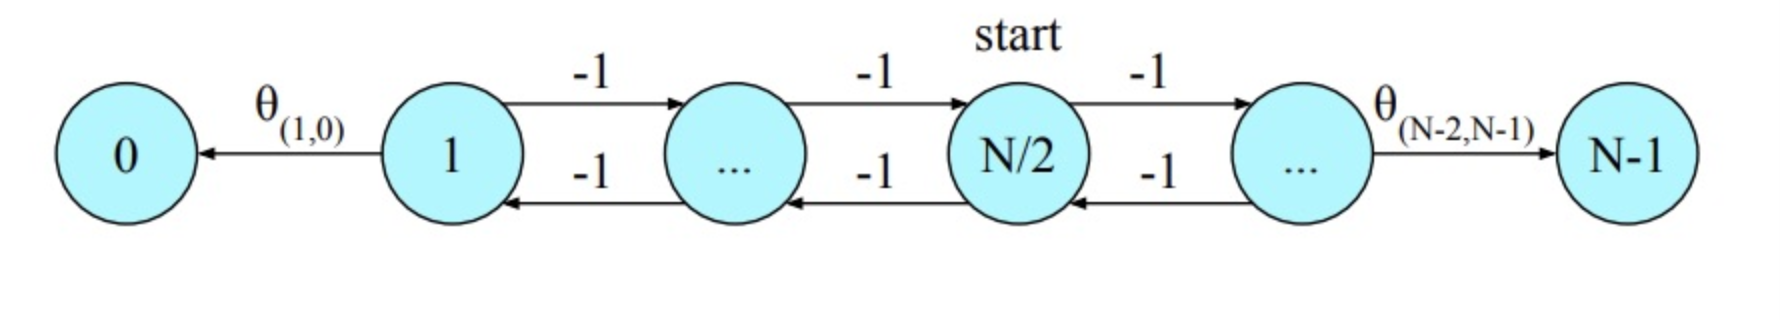
\includegraphics[scale=.25]{bipolarchain.png}

  \caption{Graph of Bipolar Chain Example.}
 \label{fig:bipolarchain}
\end{figure}
2) Parallel chains

Parallel chains are illustrated in Figure \ref{fig:parallelchains}, are constructed as a a set of singly linked lists with a common node at one end. All nodes have 0 rewards except the the end nodes. Those have  rewards that are distributed as $N(0,100+c)$ where c is a unique integer in 1 .. \# of nodes. So, you could sort them to have rewards of $N(0,101)$, $N(0,102)$ ... I didn't sort them to have more generalizable results. The actual reward obtained is a noisy (distributed normally) sample from the reward for the node.  The same chains are used for an entire run for all algorithms, but a new set of chains and rewards are sampled for each run. All transitions are deterministic.

Here is an image from the paper showing a set of parallel chains:

\begin{figure}[htbp!]
  \centering
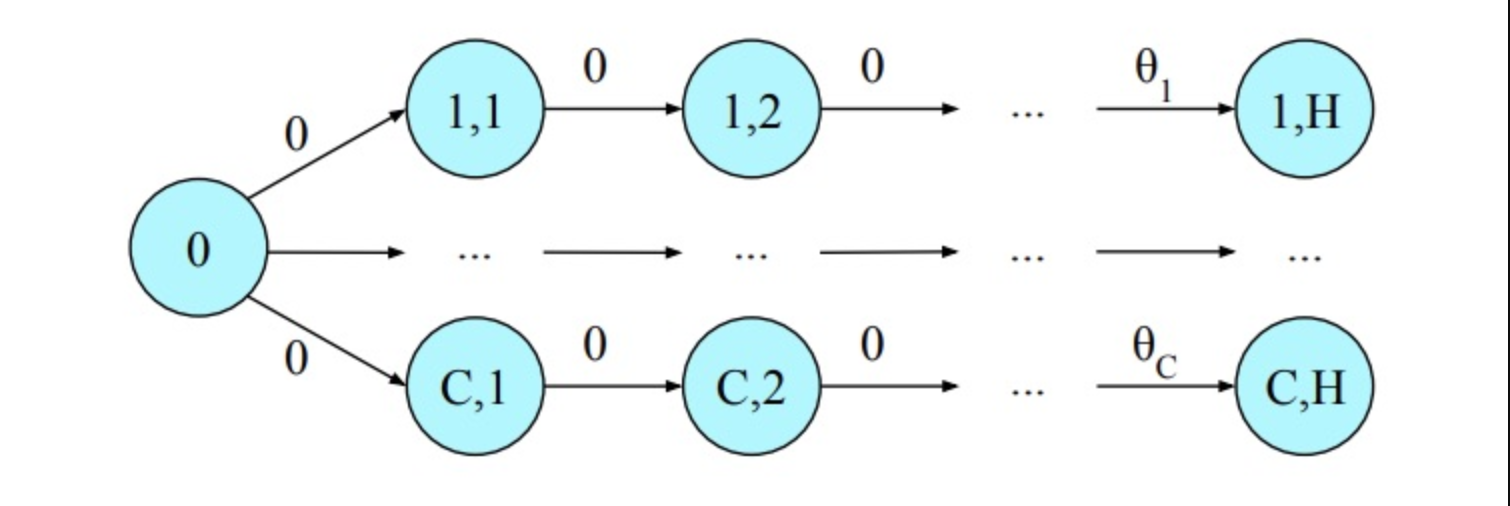
\includegraphics[scale=.25]{parallelchains.png}

  \caption{Graph of Parallel Chains Example.}
 \label{fig:parallelchains}
\end{figure}
3) Maximum reward path. 

This is constructed as a graph with nodes connected with probability p and rewards that are normally distributed. For the purposes of the example in the paper, rewards are distributed as $ln{(r_e)} | \theta_e$  \textasciitilde $N(ln{(\theta_e)} - \sigma^2/2,\sigma^2)$. The graph sample structure itself is an Erd\~os-R\'enyi graph with N =100 and probability of an edge $p=2 \frac{ln N}{N}$ Rewards are noisy, similarly to parallel chains, but with a slightly different normal distribution. Transitions between nodes, once a graph has been sampled, are deterministic., but the agent doesn't know the structure of the graph a priori. So, while transitions are deterministic, the transition matrix is not known and so, it must be discovered by the agents. The same graph is used for an entire run, but new graphs are sampled between runs.

All episodes are finite horizon.

\section{Background/Related Work}
There is the paper that is being reviewed, of course. There is also a follow on paper, that looks interesting: \cite{SCALSS} This is concerned with more scalable approaches to seed sampling. The approach is similar, but extended to allow for function approximators, such as neural networks.

In addition, there has also been some interesting work on model ensembles. This was in terms of neural networks, but that work could end up being complimentary to this: \cite{1503.02531}

Finally, I find this approach to be a bit similar to noise injection to improve the generalization of neural networks for image processing: \cite{zur2009noise} This makes me wonder if a way to remove  the need to fully solve an an MDP each time might be to view this as a way to add noise in order to generalize the learning of the agents.

\section{Approach}
Although this is a multiple agent problem, the seed sampling paper treated actions as occurring within discrete time steps, so it wasn't necessary to use a distributed (including multi-threaded) approach. So, I decided to take advantage of the fairly nice POMDPs.jl framework in Julia. 

Steps:

  \begin{itemize}
  
\item Solve the true MDP using some method. 

For the bipolar chain, I used the POMDPs.jl framework just for simulation, but I used Q-learning for solving the MDPs, that i wrote myself, but for the parallel chains and maximum reward path, I implemented a full parameterized MDP model using the POMDPs.jl interfaces for each and took advantage of the sparse value iteration solver provided. The true MDP model is used for the simulation portion and also to provide rewards mapping. 

\item Generate and solve an MDP

At the appropriate time, generate an MDP and solve it to get a policy for an episode. 

POMDPs.jl value iteration solvers don't handle stochastic rewards well (as expected), so I wrapped the true MDP function to produce the noisy response for the problem statements. I used a single MDP for the bipolar chain case, which was unknown by the agents. For parallel chains and maximum reward path, the true MDP was generated. In the case of parallel chains, random rewards were generated. In the case of maximum reward path, both the structure of the graph and the reward means were generated. This did mean that, especially in the case of a single agent, results could be very stochastic.
  
\item Run simulation

Use the POMDPs.jl methods to run a simulation on an instance of the true MDP generated for the problem, providing a function policy that matches the exploration method. For the bipolar and parallel chains, this stops as soon as it hits a goal state. For the maximum reward path a complete exploration (up to the horizon) was necessary.

Each successive time step will see a new agent started, so if there are k agents, there would be one agent started at each time step $t_1$, $t_2$, ..., $t_k$. Each agent can take X \textasciitilde Poisson(1)  actions at each time step. 
\item Repeat

Repeat for multiple runs, stepping through different \#'s of agents. Calculate the average regret.

  
 \end{itemize}
 
\subsection{Prior Updates}

  \begin{itemize}
  \item Bipolar chain
  The bipolar chain didn't really need a prior, since there were just the two big rewards: -10 and 10, and all the rest where -1. As soon as one of the endpoints was hit, the simulation could end and all agents would just go immediate towards the 10 reward.
  
  \item Parallel chains
 The prior update strategy wasn't mentioned for this problem in the paper, so  I used a standard sample gaussian prior update for this problem.
 $$\mu_{posterior} = \frac{\sigma_p^2}{(\frac{\sigma^2}{n} + \sigma_p^2)} \mu_s + \frac{\sigma_s^2}{(\frac{\sigma^2}{n} + \sigma_p^2)} \mu_p$$
 $$\sigma_{posterior} = ( \frac{1}{\sigma_p^2} + \frac{n}{\sigma^2})^{-1}$$
 where $\mu_s$ is the sample mean, $\mu_p$ is the prior mean, $\mu$ is the true mean, $\sigma_s$ is the sample standard deviation, $\sigma_p$ is the prior standard deviation, and $\sigma$ is the true standard deviation $\sigma$ and $\mu$ are assumed known, by the problem definition.
  
  \item Maximum Reward Path
  
  \cite{SeedSampling} gives the prior update directly for this problem. They used a single sample update at each time step:
  $$\mu_e = \frac{\sigma^2 \mu_e + \sigma_e^2(\ln{r_e} + \frac{\sigma^2}{2}) }{\sigma_e^2+\sigma^2}$$
  $$\sigma_e^2 = \frac{\sigma_e^2 \sigma^2}{\sigma_e^2 + \sigma^2}$$
  \end{itemize}
\subsection{Regret Calculation}
Since there were some differences between what I obtained for regret, and what the original paper obtained for regret, I thought it would be good to be clear about how I calculated regret for each problem.
\begin{itemize}
\item Bipolar chain

This problem was a little more complicated than the others, just because of how it was formulated. Since the location of the reward was considered completely known as soon as an end was reached, it was more simple to just stop the entire simulation at that point and fill in how the agents would act after that directly in the results data frame. Then the regret for an agent i would be:
$$\sum(reward_i) - N/2 $$

\item Parallel Chains

This was a little simpler. I simply took the max reward from the true MDP.
So, the regret for each agent would be (assuming c is the id of the chain with the maximum reward):
$$\argmax_c(reward) - reward_{i}$$

\item Maximum Reward Path

For this, I did something similar as for parallel chains, but for all nodes(states):
$$\sum_s \argmax_a(reward(s, a^*)) - reward(s, a) $$
\end{itemize}
\section{Experiment results}
\subsection{Bipolar Chain}
For the bipolar chain, I did runs from for $10^k$ agents for $k=1..4$. I used N=100 for the number of nodes with the horizon $H=3 \cdot \frac{N}{2}$
% latex table generated in R 3.5.2 by xtable 1.8-3 package
% Fri Mar 15 13:04:13 2019
\begin{table}[ht]
\caption{Bipolar Chain Regret per Agent Count by Algorithm Type..}
\label{bipolarregretperagentbyalgo-table}
\vskip 0.15in
\centering
\begin{tabular}{llll}
  \toprule
 & algorithm & agents & regret \\ 
  \midrule
1 & UCB &   1 & 122.00 \\ 
  2 & UCB &  10 & 120.40 \\ 
  3 & UCB & 100 & 50.22 \\ 
  4 & UCB & 1000 & 5.03 \\ 
  5 & UCB & 10000 & 0.50 \\ 
  6 & Thompson Sampling &   1 & 225.00 \\ 
  7 & Thompson Sampling &  10 & 225.00 \\ 
  8 & Thompson Sampling & 100 & 225.00 \\ 
  9 & Thompson Sampling & 1000 & 225.00 \\ 
  10 & Thompson Sampling & 10000 & 223.01 \\ 
  11 & Seed &   1 & 119.60 \\ 
  12 & Seed &  10 & 120.14 \\ 
  13 & Seed & 100 & 49.82 \\ 
  14 & Seed & 1000 & 4.97 \\ 
  15 & Seed & 10000 & 0.50 \\ 
   \bottomrule
\end{tabular}
\end{table}

\begin{figure}[htbp!]
  \centering
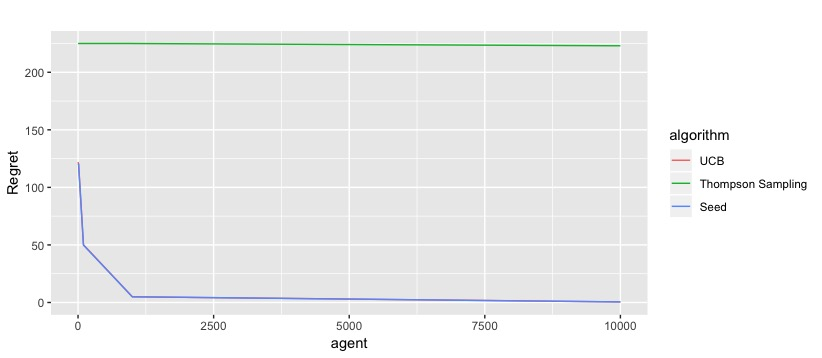
\includegraphics[scale=.3]{results_pre.jpeg}

  \caption{Bipolar Chain Regret per Agent Count by Algorithm Type.}
 \label{fig:bipolarregretperagentbyalgo}
\end{figure}
As you can see in Figure \ref{fig:bipolarregretperagentbyalgo}, and Table \ref{bipolarregretperagentbyalgo-table}, there are some small discrepancies. Thompson sampling shows an almost constant regret, only dropping at the end due to the extremely large number of agents,  which allows an agent to accidentally hit the end goal, with some higher than 0 probability. In addition, unlike in the paper, UCB was very close to the performance of seed sampling, to the point that they overlap on the graph. This could be that the paper was a little vague about the parallel UCB algorithm used. I implemented a version of UCB1 that used Q and N tables that were common across the agents. Despite this, the improvement when using seed sampling is still quite remarkable, and generally consistent with the improvement shown in the paper.


\subsection{Parallel Chains}
For parallel chains, I used the number of chains as C=10. Again running $10^k$ agents for $k=1..4$

\begin{table}[ht]
\caption{Regret per Agent Count by Algorithm Type.}
\label{pc_results_regret_by_algo-table}
\vskip 0.15in
\centering
\begin{tabular}{llll} 
\toprule 
Algorithm     & Agent Count       & Average Regret   \\ 
\midrule 
Seed Sampling     & 1       & 11.29   \\ 
Seed Sampling     & 10    & 13.49 \\ 
Seed Sampling     & 100     & 5.32  \\ 
Seed Sampling     & 1000   & 1.05  \\ 
Seed Sampling     & 10000  & 0.47  \\ 
Thompson Sampling & 1          & 14.27 \\ 
Thompson Sampling & 10       & 12.71   \\ 
Thompson Sampling & 100    & 5.66  \\ 
Thompson Sampling & 1000    & 1.07  \\ 
Thompson Sampling & 10000  & 0.47 \\ 
UCB               & 1         & 18.81  \\ 
UCB               & 10       & 17.15 \\ 
UCB               & 100      & 10.05 \\ 
UCB               & 1000    & 1.45 \\ 
UCB               & 10000  & 0.49      \\ 
\bottomrule 
\end{tabular}
\end{table}


\begin{figure}[htbp!]
  \centering
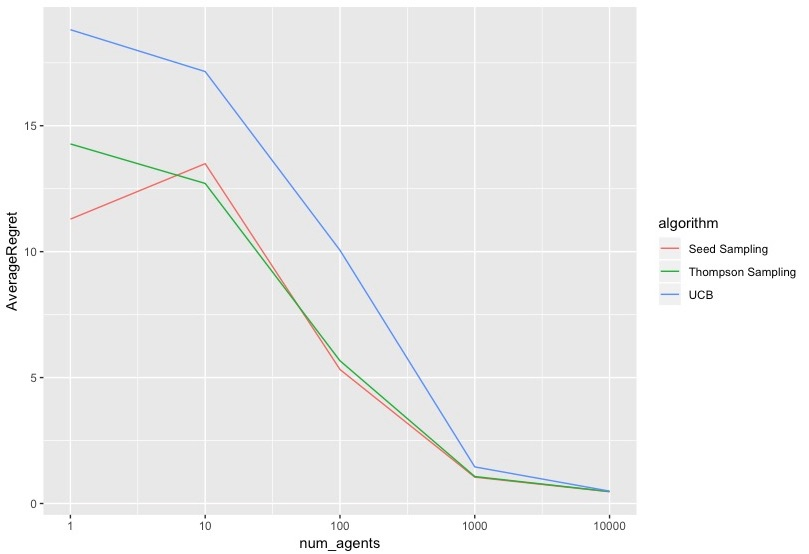
\includegraphics[scale=.3]{pc_results_regret_by_algo.jpg}

  \caption{Parallel Chain Regret per Agent Count by Algorithm Type.}
 \label{fig:pc_results_regret_by_algo}
\end{figure}
As you can see in Figure  \ref{fig:pc_results_regret_by_algo}, the results again were fairly close to the paper. My results did converge   faster for UCB.  As I pointed out above, the exact algorithm they used for UCB wasn't mentioned in the paper, so it could be due to a limitation of the algorithm they chose. For this problem, since the rewards were normally distributed, I just used a 4 sigma upper control bound.

What really makes the results stand our for me is Figure \ref{fig:pc_max_time_per_ag_by_algo}.  Despite having comparable performance in terms of average regret, seed sampling is computationally much more efficient than Thompson sampling. 
\begin{figure}[htbp!]
  \centering
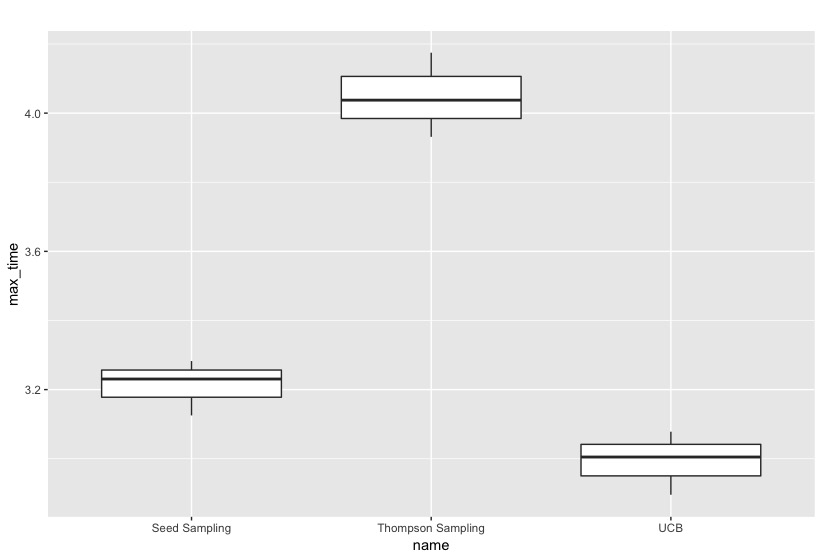
\includegraphics[scale=.3]{pc_max_time_per_ag_by_algo.jpg}

  \caption{Parallel Chain Time (in minutes) per Run for 10000 Agents by Algorithm Type.}
 \label{fig:pc_max_time_per_ag_by_algo}
\end{figure}


\subsection{Maximum Reward Path}
For maximum reward path I used number of nodes N=100,  with a horizon of H=10.

\begin{figure}[htbp!]
  \centering
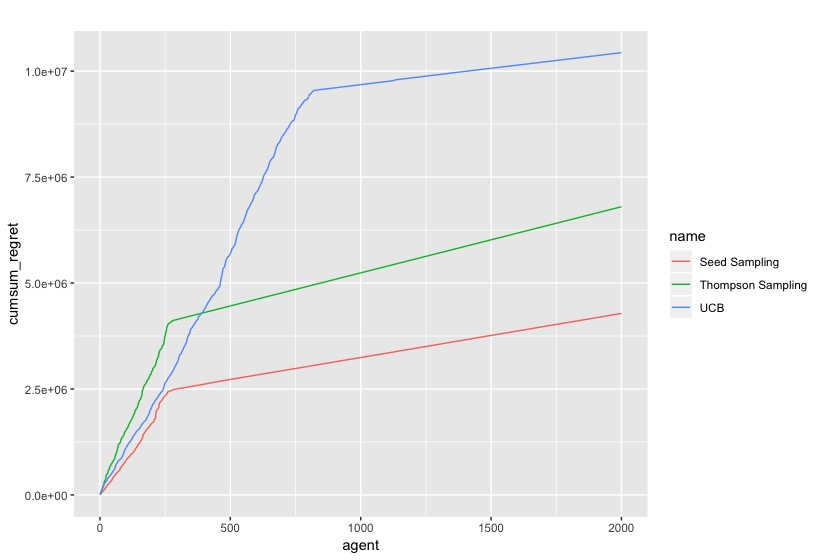
\includegraphics[scale=.3]{mr_regret_per_ag_per_algo.jpg}
  \caption{Maximum Reward Path Regret per Agent Count by Algorithm Type.}
 \label{fig:mr_regret_per_ag_per_algo}
\end{figure}
For this problem, two of the algorithms were switched in performance for me, versus this paper. UCB was performing worse than Thompson sampling.  To be honest, I didn't really understand why UCB performed better that Thompson sampling in the paper. I would expect that the lack of exploration that caused the difficulties that UCB had in terms of a lack of diversity in exploration in the parallel chains scenario would carry over to this one. 

\begin{figure}[htbp!]
  \centering
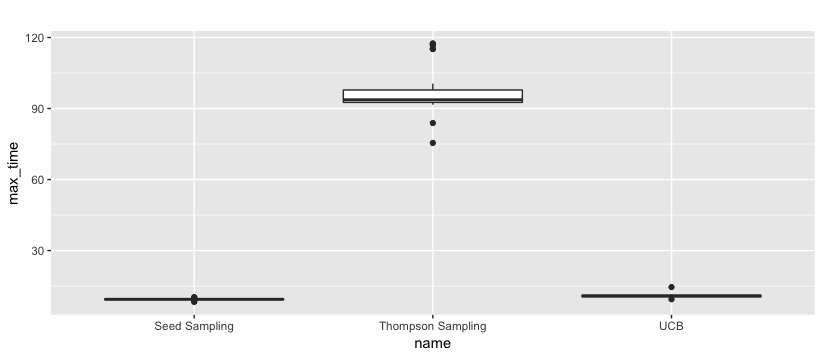
\includegraphics[scale=.3]{mr_max_time_per_ag_by_algo.jpg}

  \caption{Maximum Reward Path Time (in minutes) per Run for 2000 Agents by Algorithm Type.}
 \label{fig:mr_max_time_per_ag_by_algo}
\end{figure}
This graph was really interesting.  You can really see the advantages of seed sampling over Thompson sampling in terms of computation. The cost of solving an MDP on every step is extremely expensive. Since the horizon was 10 for this problem, you can see exactly that magnitude of an increase in the time taken by Thompson sampling. To the point that it would be very prohibitive for large problems. 

In the scalable version of this paper,  they mention using ensembles of solved MDPs to additionally reduce the amount of computation, since that appears to be the most time consuming portion:  \cite{SCALSS} The mechanism wasn't specified, but the idea in that situation seems to be to solve models without the seed, then apply the seed to the solved model. This would imply that the seeding would not be included in the value function itself, and so part of the discounted value, but instead would be applied post hoc to a completed value function a bit like how UCB1 works, a type of random exploration bonus.  This is the reverse of the procedure from the \citep{SeedSampling} paper, which sampled an MDP as a function of the seed.  

\section{Conclusion}
I was able to replicate the findings in the paper. The results aren't exactly the same, but that isn't too surprising given that they aren't specific about the algorithms they compared against. What was really impressive was the gain in computational efficiency by reducing how often MDPs need to be solved. In all cases, seed sampling was much faster than thompson sampling, scaling as the number of episodes vs. the number of time steps. Yet, seed sampling retained much of the benefits of Thompson sampling in terms of providing exploration diversity.


As mentioned above, the ideas here seem to be similar to adding noise to training images to improve generalization. It makes me think that it's likely this idea could be taken out of the Bayesian context and applied to algorithms like UCB1 or MSIE-EB, especially if the PAC guarantees of MSIE-EB could be retained. It seems likely that such a method would use something similar to how you would implement the ensembles mentioned in the \cite{SCALSS} paper.

Overall, seed sampling seems like it would be a very useful way to enhance diversity in exploration while avoiding some of the degenerative behavior of Thompson sampling in problems that have sparse rewards.
\section{References}

\bibliography{project_update}
\bibliographystyle{icml2018}

\section{Source Code}
The source code I used is at \href{https://github.com/efancher/cs234_work_final_project}{Source Code}: \verb|https://github.com/efancher/cs234_work_final_project|. The repository is public. I included a (very) short readme: Readme.txt that explains the different files.

\section{Collaborators}
This was a solo project. So, just Edward Fancher - efancher.


\end{document}


% This document was modified from the file originally made available by
% Pat Langley and Andrea Danyluk for ICML-2K. This version was created
% by Iain Murray in 2018. It was modified from a version from Dan Roy in
% 2017, which was based on a version from Lise Getoor and Tobias
% Scheffer, which was slightly modified from the 2010 version by
% Thorsten Joachims & Johannes Fuernkranz, slightly modified from the
% 2009 version by Kiri Wagstaff and Sam Roweis's 2008 version, which is
% slightly modified from Prasad Tadepalli's 2007 version which is a
% lightly changed version of the previous year's version by Andrew
% Moore, which was in turn edited from those of Kristian Kersting and
% Codrina Lauth. Alex Smola contributed to the algorithmic style files.
